\documentclass[conference]{IEEEtran}
\IEEEoverridecommandlockouts

\usepackage{amsmath,amssymb,amsfonts}
\usepackage{graphicx}
\usepackage{booktabs}
\usepackage{array}
\newcolumntype{L}[1]{>{\raggedright\arraybackslash}p{#1}}
\usepackage{multirow}
\usepackage{algorithm}
\usepackage{algpseudocode}
\usepackage{xcolor}
\usepackage{url}
\usepackage[hidelinks]{hyperref}
\usepackage{cite}

\graphicspath{{figures/}}
% Many full-width figures: let them share pages so they stay near their text.
\renewcommand{\topfraction}{0.9}
\renewcommand{\dbltopfraction}{0.9}
\renewcommand{\textfraction}{0.07}
\renewcommand{\floatpagefraction}{0.75}
\renewcommand{\dblfloatpagefraction}{0.75}
\setcounter{topnumber}{3}
\setcounter{dbltopnumber}{3}
\setcounter{totalnumber}{5}
\newcommand{\awr}{\textsc{ActiveWR}}
\newcommand{\pp}{\,pp}
\newcommand{\ci}[2]{[#1,\,#2]}
% Per-decision timing, paper/figures/decision_timing.json (6 validation games, 745 decisions, 1 CPU thread)
\newcommand{\searchms}{213}
\newcommand{\cnnms}{1.9}
\newcommand{\speedratio}{115}

\begin{document}

\title{Winning Is Not Killing: Active Win Rate and Expert Iteration with a Network-Free Kill-Search in Bomberman}

% Double-blind submission: replace with the author block for the camera-ready version.
\author{\IEEEauthorblockN{Anonymous Author(s)}
\IEEEauthorblockA{Affiliation withheld for review}}

\maketitle

\begin{abstract}
Agents for Bomberman-like games are usually ranked by win rate, yet a game can be won because the opponent destroys itself or is caught by a shrinking arena. We define \emph{active win rate} (\awr{}), the share of games won with at least one kill credited to the learner's own bomb, and use it to study how a hand-written kill-search that uses no neural network can be turned into a fast neural policy on consumer hardware. In a $9\times9$ one-versus-one Bomberman game against a fixed rule-based bot, policy-gradient training with a safety mask and auxiliary teachers reaches 40.0--51.0\% \awr{}, and more than a dozen standard refinements fail a gate fixed before testing. A kill-search that looks one, two or three learner moves ahead over 12 ticks, with the opponent modelled as the rule-based bot, lifts the same network to 64.75, 82.0 and 94.0\%. Used as a sparse auxiliary loss inside reinforcement learning the search does not help ($-2.75$\pp{}), whereas dense distillation of its labels on decision states does ($+16.25$\pp{}). Three rounds of expert iteration, each distilling the current student plus a deeper search, produce S3: a plain convolutional policy at 92.25\% \awr{}, 0.75\pp{} below its search teacher with a confidence interval of \ci{-4.0}{+2.5} that includes zero, using one forward pass per move. Interventions that add 3.75--16\pp{} of win rate add no \awr{}. Against frozen neural opponents most games end in draws; with a correct opponent model the search finds a kill plan in only 15.9\% of them, so most of these draws seem to come from the game rather than from missed chances. All tests use single-use seeds, a paired bootstrap over boards and acceptance gates fixed in advance.
\end{abstract}

\begin{IEEEkeywords}
Bomberman, Pommerman, reinforcement learning, expert iteration, policy distillation, game-tree search, evaluation metrics
\end{IEEEkeywords}

% =====================================================================================
\section{Introduction}

Deep reinforcement learning (RL) reaches human or grandmaster level in Atari and StarCraft~II~\cite{mnih2015dqn,vinyals2019alphastar}, but with compute far beyond a single consumer machine. Bomberman, and its research variant Pommerman~\cite{resnick2018pommerman}, is a hard test for model-free RL at small scale. A bomb placed at random kills its owner about 40\% of the time~\cite{gao2019hard}, so exploration is suicidal; the reward for a kill arrives many steps after the decision that made it; and the decisive moments are rare. Large RL efforts needed hundreds of CPUs~\cite{peng2018continual} or long population-based training~\cite{huynh2024}, and still lost to search-based agents~\cite{osogami2019,huynh2024}. The strongest agents combine an action filter or a search with learning~\cite{gao2019skynet,osogami2019,weil2023}.

A second problem is less visible: \emph{how agents are scored}. Several groups noticed that an agent can collect wins when the opponent kills itself~\cite{gao2019skynet,kartal2018demonstrator,huynh2024,weil2023}, but results are still reported as win rate (WR) or tournament points. We met this problem directly. An early checkpoint of ours won 52.5\% of 40 four-player games while killing nobody with its own bombs, and a mask margin that raised WR by 10.75\pp{} left the kill-based win rate unchanged (Section~\ref{sec:rq1}).

This paper reports a controlled study, run on consumer hardware, of how to get a fast neural Bomberman agent that wins by killing. We make the following contributions.

\begin{itemize}
\item \textbf{C1, a metric.} We define \awr{}, the probability of winning \emph{and} killing at least one opponent with one's own bomb, with kill credit assigned to the bomb's owner through chain explosions. Win rate overstates three of our interventions by 3.75--16\pp{} (Fig.~\ref{fig:wr}).
\item \textbf{C2, three uses of the same search.} With one kill-search, we compare (a) sparse search labels as an auxiliary RL loss, (b) search at play time and (c) dense distillation of search labels. Only (b) and (c) help ($-2.75$, $+16.5$ and $+16.25$\pp{}). This tests the two future directions proposed by Kartal et al.~\cite{kartal2018demonstrator}.
\item \textbf{C3, expert iteration with a network-free expert.} Three rounds of ``student plus deeper search $\rightarrow$ distil'' raise a plain CNN from 48.25\% (best RL policy) to 92.25\% \awr{}; the student--teacher gap shrinks from $-3.75$ to $-3.5$ to $-0.75$\pp{} while the teachers get stronger.
\item \textbf{C4, controlled negative results.} We report gated, single-test-seed results for generalized advantage estimation (GAE), PPO clipping, advantage normalisation, reward changes, curricula, sudden-death training, group-relative advantages and KL-anchored RL after distillation. None passes.
\item \textbf{C5, a draw analysis.} Strong agents draw most games against each other. A probe with the correct opponent model finds a kill plan in 15.9\% \ci{9.9}{22.7} of such draws, against 90.3\% under the rule-bot assumption, and the wrong opponent model costs 33\pp{}.
\item \textbf{C6, transfer to a larger board.} Re-distilling on $11\times11$ adds $+41.0$\pp{} \ci{34.5}{47.25} against the rule bot but only $+3.83$\pp{} \ci{1.92}{5.83} against neural opponents.
\end{itemize}

Fig.~\ref{fig:pipeline} summarises the path from the first RL checkpoint to the final agent. Each building block (masked policy gradient, search, distillation, group-relative advantages) is known; the contribution is the metric, the controlled comparison under a fixed protocol, and the analysis of where the remaining draws come from.

\begin{figure*}[t]
\centering
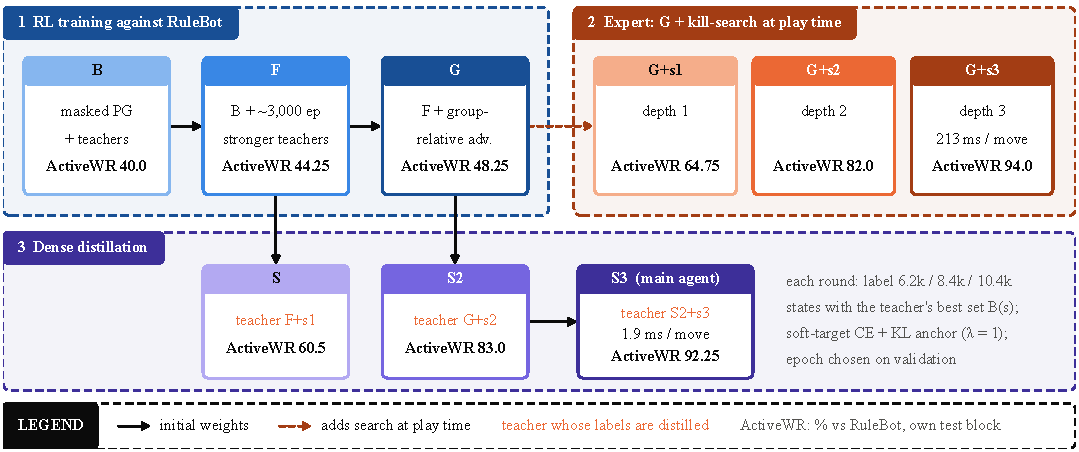
\includegraphics[width=\textwidth]{fig_pipeline.pdf}
\caption{Path from the first RL checkpoint to the final agent. Panel 1: RL-trained CNNs (blue). Panel 2: G with kill-search at play time (orange, the expert); the dashed arrow adds search without changing any weights. Panel 3: distilled CNN students (violet). Black arrows give the initial weights of each model; the orange label names the teacher whose search labels it is trained on, so S2 starts from G, not from S. Each agent keeps the same colour in every figure. Numbers are \awr{} (\%) against RuleBot under schedule E, each on the model's own single-use test block (Table~\ref{tab:main}); only same-block comparisons are inferential.}
\label{fig:pipeline}
\end{figure*}

% =====================================================================================
\section{Related Work}

\textbf{RL in Bomberman and Pommerman.} Pommerman~\cite{resnick2018pommerman} made Bomberman a multi-agent benchmark. Without action filtering, PPO learned nothing in five days; with a filter it learned~\cite{gao2019hard}. Skynet~\cite{gao2019skynet} combined PPO, an action filter and reward shaping, and observed that wins often came from opponents killing themselves. Imitation then RL suffered catastrophic forgetting~\cite{meisheri2019}; curriculum and population-based self-play still lost 70--95\% of games to search agents after 200 million steps~\cite{huynh2024}. Backplay~\cite{resnick2018backplay} starts episodes from the end of a demonstration and moves the start backwards, and continual match training used 220 CPUs and 32 GPUs~\cite{peng2018continual}. For classic Bomberman, Q-learning with a multi-layer perceptron was used to compare exploration rules~\cite{kormelink2018}, and imitation followed by PPO was applied to a Unity version~\cite{goulart2019}.

\textbf{Search in Pommerman.} The NeurIPS 2018 winner used depth-limited tree search with \emph{pessimistic} opponent scenarios and beat the best RL agents in 87.1\% of 22{,}500 games~\cite{osogami2019}. Statistical forward planning (MCTS, RHEA) produced 59--84\% draws between strong planners~\cite{perezliebana2019}. MCTS with learned opponent models can turn defensive and slow~\cite{weil2023}; mixtures of phase experts help MCTS by 5--11\% in Pommerman~\cite{helfenstein2024}. Opponent modelling inside the policy was studied by DOMAC~\cite{sun2022domac}.

\textbf{Search as a teacher.} Guo et al.~\cite{guo2014uct} trained real-time Atari CNNs on UCT decisions. Expert iteration (ExIt)~\cite{anthony2017exit} and AlphaGo Zero / AlphaZero~\cite{silver2017agz,silver2017alphazero} alternate a search expert and a network apprentice, with the network guiding the search. In Pommerman, MCTS was used as a demonstrator inside A3C~\cite{mnih2016a3c} on an $8\times8$ mini-board~\cite{kartal2018demonstrator,kartal2019safer,kartal2019guidance}; those authors proposed, but did not test, calling the demonstrator only in relevant states and storing its actions in a buffer. Distillation~\cite{hinton2015distill,rusu2016distill,czarnecki2019distill}, DAgger~\cite{ross2011dagger} and kickstarting~\cite{schmitt2018kickstart} give the supervised side of our method.

\textbf{Safety and evaluation.} Masking invalid actions in the logits keeps a valid policy gradient~\cite{huang2022masking}; shields block unsafe actions with minimal interference~\cite{alshiekh2018shield}. Only potential-based shaping preserves optimal policies~\cite{ng1999shaping}, and dense rewards should be annealed~\cite{bansal2018emergent}. RL results need confidence intervals over independent units and several runs~\cite{henderson2018matters,agarwal2021precipice}; we use Efron's bootstrap~\cite{efron1979bootstrap} over paired boards. Table~\ref{tab:related} positions this work.

\begin{table}[t]
\centering
\caption{Positioning against the closest work.}
\label{tab:related}
\footnotesize
\setlength{\tabcolsep}{2pt}
\begin{tabular}{@{}L{0.2\columnwidth}L{0.25\columnwidth}L{0.27\columnwidth}L{0.22\columnwidth}@{}}
\toprule
Work & Learning & Search & Metric \\
\midrule
\cite{gao2019skynet,gao2019hard} & PPO + action filter & -- & WR \\
\cite{osogami2019} & -- & depth 1, pessimistic & WR, draws \\
\cite{kartal2018demonstrator,kartal2019guidance} ($8\times8$) & A3C + MCTS demonstrator & shallow MCTS & reward curve \\
\cite{weil2023} & ExIt (AlphaZero-style) & MCTS + network & WR \\
\cite{huynh2024} & PPO, curriculum, PBT & -- & WR, enemies killed \\
\textbf{Ours} ($9\times9$, $11\times11$) & PG, dense distillation & network-free kill-search & \textbf{\awr{}}, paired CI \\
\bottomrule
\end{tabular}
\end{table}

% =====================================================================================
\section{Problem Setting}
\label{sec:setting}

\textbf{Game.} We use a NumPy re-implementation of Pommerman-style free-for-all Bomberman. The board is $9\times9$ with a border and pillars of rigid walls on (even, even) cells; 70\% of the other free cells hold wooden walls, except $3\times3$ spawn zones. Two agents start in opposite corners. Actions are STOP, four moves and BOMB. A bomb explodes after 8 steps into a cross-shaped blast (initial range 2), destroys wooden walls (a power-up appears with probability 0.3: extra bomb or longer range), kills agents in the blast and chains into other bombs. Flames last 2 steps. A game ends when at most one agent is alive or after 500 steps (draw). Fig.~\ref{fig:game} shows a game in progress. Our default sudden-death schedule E closes the arena from the border inwards from step 475 every 25 steps, with a 40-step warning.

\textbf{Observation.} Each agent sees 13 $9\times9$ planes (Fig.~\ref{fig:obs}, Appendix): rigid and wooden walls, bomb timers, flames, two power-up types, own and opponent positions, three constant planes (free bomb slots, capacity, range), the inverse time until each cell is hit by a forecast blast including chains, and the sudden-death warning.

\textbf{Safety mask and opponent.} Every agent acts through the same safe-action mask $m(s)\in\{0,1\}^6$, which removes moves into cells that a forecast blast will reach before the agent can leave, and bombs without an escape route; it has fallbacks so that at least one action stays legal. The standard opponent is a rule-based bot (RuleBot) that dodges, collects items, attacks with the correct blast range and uses the same mask; when none of its rules applies it picks a random safe move, so its play is stochastic. RuleBot is kept fixed throughout.

\begin{figure*}[t]
\centering
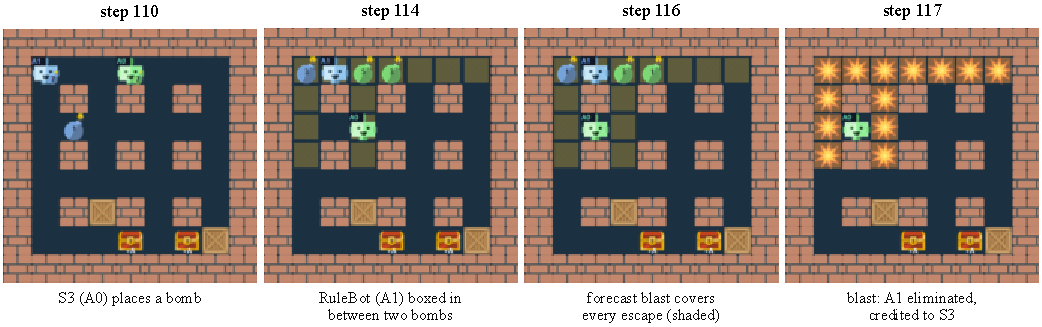
\includegraphics[width=\textwidth]{fig_gameplay.pdf}
\caption{Four frames of a real game, captured from the game's own viewer: S3 (A0, green) against RuleBot (A1, blue) on validation board 21000. The number on a bomb is its fuse; shaded cells are the forecast blast area (plane 11 in Fig.~\ref{fig:obs}), shown in the middle two frames. S3's bomb placed at step 110 and a second one at step 112 box RuleBot in next to its own bomb; the chain explosion at step 117 kills it, and the kill is credited to S3, so this game counts as an active win.}
\label{fig:game}
\end{figure*}

\textbf{Metric.} Let $W$ be the event that the learner is the last agent alive and $K$ the event that at least one opponent died in a blast credited to a learner bomb (credit follows the owner of the bomb that started a chain). We report
\begin{equation}
\awr{}(\pi)=\Pr_{\pi}\left[\,W \wedge K\,\right],
\end{equation}
and decompose every evaluation into active wins, passive wins (opponent self-kill), ring wins (opponent caught by sudden death), draws, learner self-kills and other losses. WR $=\Pr[W]$ is reported only as a secondary number.

% =====================================================================================
\section{Method}

\subsection{Network}
All agents share one actor--critic CNN (Fig.~\ref{fig:arch}): three $3\times3$ convolutions (32, 64, 64 channels, padding 1, ReLU), a 256-unit fully connected layer, a 6-way actor head and a scalar critic head, 1{,}388{,}359 parameters in total. The policy masks logits before the softmax,
\begin{equation}
\pi_\theta(a\mid s)=\frac{m_a(s)\exp z_a(s)}{\sum_b m_b(s)\exp z_b(s)},
\end{equation}
implemented as \texttt{masked\_fill}$(\neg m,-10^9)$ both when sampling and inside every loss, which keeps the policy gradient valid~\cite{huang2022masking}. Actions are \emph{sampled}; on validation, argmax play lowered F's \awr{} by 9.25\pp{} \ci{-16.0}{-2.5} and raised draws by 7.5\pp{} \ci{1.25}{13.75}. We did not diagnose why; a likely reason is that a deterministic policy can repeat the same move sequence, which sampling breaks.

\begin{figure*}[t]
\centering
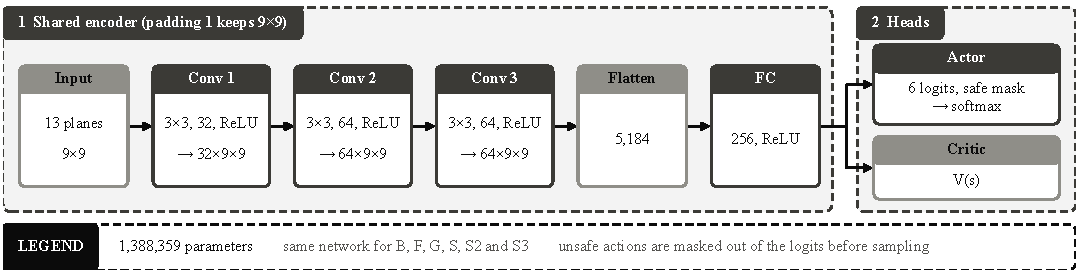
\includegraphics[width=\textwidth]{fig_architecture.pdf}
\caption{Actor--critic network used by every agent in this paper (B, F, G, S, S2, S3). The safe-action mask is applied to the logits.}
\label{fig:arch}
\end{figure*}

\subsection{Stage 1: masked policy gradient with auxiliary teachers}
The RL stage trains against RuleBot with Monte-Carlo returns $G_t=\sum_{k}\gamma^k r_{t+k}$, $\gamma=0.99$, and a learned baseline (REINFORCE with baseline~\cite{williams1992reinforce,sutton2018rl}; GAE~\cite{schulman2016gae} and PPO clipping~\cite{schulman2017ppo} were tested as variants):
\begin{multline}
\mathcal{L}_{\mathrm{RL}}=\tfrac{1}{T}\textstyle\sum_t\Bigl[-\log\pi_\theta(a_t\mid s_t)\,\hat A_t+c_v\hat A_t^{\,2}\\
-c_e\,\mathcal{H}\bigl(\pi_\theta(\cdot\mid s_t)\bigr)\Bigr]+\textstyle\sum_k c_k\,\mathcal{L}^{\mathrm{teacher}}_k,
\end{multline}
with $\hat A_t=G_t-V_\phi(s_t)$ (detached in the policy term). The auxiliary terms are cross-entropy losses towards four rule-based teachers (escape, combat, navigation, ring safety) with weights $0.5, 0.9, 0.4, 0.6$; the attack-related weights are multiplied by 1.75 after step 350 of a game. Rewards are event-based: $-0.001$ per step alive, $+0.05$ per useful item, $+0.15$ per wooden wall destroyed, $+4$ per credited kill, $-1$ on death and an extra $-1.5$ for a self-kill. The environment's $+10$ for being last alive is kept only for active wins; for passive wins it is cancelled, which aligns the return with \awr{} rather than shaping it.

\textbf{Group-relative advantage.} Because a game of about 230 steps contains on average only about 2.2 steps where the actions' search scores differ, and about 1.25 where some action leads to a kill, we also tried a GRPO-like update~\cite{shao2024grpo} at \emph{decisive} states, where the kill-search below finds a credited kill within 12 ticks. From each such state the current policy is replayed $K=16$ times for $H=20$ ticks against fresh RuleBots, with outcome $o_k\in\{+1\ \text{(credited kill)},-1\ \text{(death)},0\}$ and advantage $A_k=o_k-\bar o$; the loss $-\frac1K\sum_k A_k\sum_{t}\log\pi_\theta(a_{k,t}\mid s_{k,t})$ is added with weight 4 (at most 6 states per episode, at least 4 steps apart). The resulting checkpoint G is our best RL policy.

\subsection{Stage 2: network-free kill-search}
The expert is a short-horizon search that uses no network (Algorithm~\ref{alg:search}). For each legal first action, a copy of the game is simulated for 12 ticks (bomb fuse 8 + flame 2 + slack): the opponent plays RuleBot and the learner only dodges after its first action. A rollout scores $+1$ if an opponent dies from a learner bomb while the learner is alive, $-1$ if the learner dies, else 0. Depth $d=2$ or 3 extends the search to two or three learner moves before dodging, and is only expanded when no shorter plan kills. The search is skipped unless an opponent is within Manhattan distance 6 (no kill fits the horizon beyond it). The CNN's sampled action is kept unless another action scores strictly higher, so the search only changes decisions that matter.

\begin{algorithm}[t]
\caption{Kill-search of depth $d$ (play time)}
\label{alg:search}
\small
\begin{algorithmic}[1]
\Require state $s$, learner $i$, mask $m$, CNN action $a_0$, depth $d$, horizon $H=12$
\If{no opponent within distance 6} \Return $a_0$ \EndIf
\For{$a$ with $m_a(s)=1$}
  \State $v_1(a)\gets$ \Call{Rollout}{$s,[a],H$} \Comment{RuleBot opponent, learner dodges}
\EndFor
\If{$\max_a v_1(a)>v_1(a_0)$} \Return $\arg\max_a v_1(a)$ \EndIf
\For{$\ell=2,\dots,d$} \Comment{only if no shorter kill}
  \For{safe action prefixes $(a,b_2,\dots,b_\ell)$}
    \State $v_\ell(a)\gets\max$ \Call{Rollout}{$s,(a,b_2,\dots,b_\ell),H$}
  \EndFor
  \If{some $v_\ell(a)>0$ and $v_\ell(a_0)\le 0$} \Return first move of a kill plan \EndIf
\EndFor
\State \Return $a_0$
\end{algorithmic}
\end{algorithm}

\subsection{Stage 3: dense distillation and expert iteration}
\textbf{Data.} The teacher (current student + kill-search of depth $d$) plays 3{,}000 games against RuleBot on fresh boards (sudden death E in 75\% of games). At every learner step the search scores all legal actions; a \emph{decision state} is one where the scores differ. Its target spreads mass uniformly over the best set $B(s)$:
\begin{equation}
q(a\mid s)=\frac{\mathbb{1}[a\in B(s)]}{|B(s)|},\qquad B(s)=\arg\max_{a:\,m_a(s)=1} v(a).
\end{equation}
With probability 0.05 an ordinary state is also stored as an \emph{anchor}, with the reference logits of the starting network $\pi_{\mathrm{ref}}$. Rounds 1--3 collected 6{,}171, 8{,}449 and 10{,}425 decision states and up to 29{,}483 anchors.

\textbf{Loss.} The student starts from the previous network and minimises
\begin{multline}
\mathcal{L}_{\mathrm{distill}}=\mathbb{E}_{s\in\mathcal{D}_{\mathrm{dec}}}\Bigl[-\textstyle\sum_a q(a\mid s)\log\pi_\theta(a\mid s)\Bigr]\\
+\lambda\,\mathbb{E}_{s\in\mathcal{D}_{\mathrm{anc}}}\mathrm{KL}\bigl(\pi_{\mathrm{ref}}(\cdot\mid s)\,\Vert\,\pi_\theta(\cdot\mid s)\bigr),
\end{multline}
with $\lambda=1$, Adam, learning rate $10^{-4}$, batch 256, 8 or 16 epochs. A board-level 10\% split is held out to monitor accuracy, and the epoch is chosen by \awr{} on validation seed 21000 before any test. We do not augment with rotations: on 6{,}171 audited states only 79.2\% kept the same best-action set after a symmetry transform, because the search and RuleBot break ties asymmetrically (cf.\ AlphaZero dropping augmentation for asymmetric games~\cite{silver2017alphazero}).

\textbf{Iteration.} Round 1 distils F + depth-1 search into S (from F); round 2 distils G + depth-2 into S2 (from G); round 3 distils S2 + depth-3 into S3 (from S2). Unlike ExIt~\cite{anthony2017exit}, the expert never uses the network's prior or value; the student improves only because the expert also contains the previous student's own moves where the search is indifferent, which keeps the data close to the student's state distribution~\cite{ross2011dagger}.

\begin{table}[t]
\centering
\caption{Main settings (defaults; one train seed per arm).}
\label{tab:hyper}
\footnotesize
\setlength{\tabcolsep}{3pt}
\begin{tabular}{@{}L{0.24\columnwidth}L{0.72\columnwidth}@{}}
\toprule
RL (Stage 1) & Adam, lr $2.5\times10^{-5}$, $\gamma=0.99$, $c_v=0.5$, $c_e=0.0075\rightarrow0.0015$; 3{,}000 episodes per arm, validation every 500 (400 games) \\
Group advantage & $K=16$, $H=20$, weight 4, $\le$6 states/episode \\
Kill-search & horizon 12 ticks, reach 6, depth 1/2/3, opponent model RuleBot \\
Distillation & 3{,}000 teacher games, anchors 5\%, $\lambda=1$, lr $10^{-4}$, batch 256 \\
Evaluation & 200 boards $\times$ 2 corners, 500 steps, schedule E, sampled actions \\
Statistics & paired bootstrap over boards, $10^4$ resamples, seed 20261014 \\
Hardware & consumer GPUs (RTX 3050/4060) for updates; CPU for search and tests \\
\bottomrule
\end{tabular}
\end{table}

% =====================================================================================
\section{Evaluation Protocol}
\label{sec:protocol}

Every experiment follows the same pre-specified protocol (fixed in our repository before each run, not in a public registry). (i) Configuration, source hashes and the selection rule are written before training. (ii) Checkpoints are selected only on validation seed 21000. (iii) The selected models are tested \emph{once} on a fresh block of 200 boards, each played from both corners (400 games per model); a test seed block is never reused. (iv) Models are compared with a paired bootstrap~\cite{efron1979bootstrap}: for board $b$, $d_b$ is the difference in \awr{} averaged over the two corners, $\hat\Delta=\bar d$, and the 95\% percentile interval comes from $10^4$ resamples of boards. (v) A change is accepted only if $\hat\Delta\ge+5$\pp{}, the lower CI bound is above zero, and self-kills do not rise by more than 1\pp{}. Failing results are reported as such. A single 400-game test block of the same pair varies by about $\pm5$\pp{} across blocks (e.g.\ $-6.5$, $+3.5$, $+3.0$ for one pair on three blocks; $0.0$ \ci{-3.75}{3.75} pooled over 600 boards), which is why the gate requires both a margin and a positive lower bound. We ask five research questions:
\textbf{RQ1} how much does WR misjudge agents? \textbf{RQ2} which use of a search transfers its strength to a CNN? \textbf{RQ3} how close can expert iteration with a network-free expert bring a CNN to the search? \textbf{RQ4} why do RL refinements fail from a good policy? \textbf{RQ5} are draws between strong agents missed chances or structural?

% =====================================================================================
\section{Results}

\begin{table*}[t]
\centering
\caption{Main results against RuleBot ($9\times9$, 1v1, schedule E, 400 test games per model). Each row uses the model's own single-use test block; rows on the same block can be compared directly (Fig.~\ref{fig:forest}). CI: 95\% bootstrap over boards. $^\ast$B's first confirmation test (block 32000) was run before sudden death existed and gave 32.75 \ci{28.25}{37.5} \awr{} with 60.5\% draws; the row shown is B under schedule E on the cross-check block 60000.}
\label{tab:main}
\small
\resizebox{\textwidth}{!}{%
\begin{tabular}{@{}llrrrrrrr@{}}
\toprule
Agent & Description & Test block & \awr{} \% [95\% CI] & WR \% & Passive/ring win \% & Draw \% & Self-kill \% & Mean steps \\
\midrule
B$^\ast$ & masked PG + teachers & 60000 & 40.0 \ci{35.0}{45.0} & 64.0 & 24.0 & 22.5 & 0.5 & 357 \\
F & B + $\sim$3{,}000 RL episodes & 43000 & 44.25 \ci{39.25}{49.25} & 63.5 & 19.25 & 25.0 & 1.0 & 340 \\
G & F + group-relative advantage & 46000 & 48.25 \ci{43.5}{53.25} & 69.0 & 20.75 & 23.25 & 0.75 & 335 \\
\midrule
G+s1 & G + kill-search, depth 1 & 46000 & 64.75 \ci{60.25}{69.25} & 84.0 & 19.25 & 15.25 & 0.0 & 287 \\
G+s2 & G + kill-search, depth 2 & 47000 & 82.0 \ci{78.25}{85.75} & 93.75 & 11.75 & 5.75 & 0.0 & 208 \\
G+s3 & G + kill-search, depth 3 & 49000 & \textbf{94.0} \ci{91.75}{96.25} & 99.5 & 5.5 & 0.25 & 0.0 & 114 \\
\midrule
S & distil F+s1 (round 1) & 43000 & 60.5 \ci{55.25}{65.75} & 78.5 & 18.0 & 18.0 & 1.0 & 279 \\
S2 & distil G+s2 (round 2) & 48000 & 83.0 \ci{79.5}{86.5} & 90.25 & 7.25 & 7.0 & 0.25 & 211 \\
S3 & distil S2+s3 (round 3) & 57000 & \textbf{92.25} \ci{89.5}{94.75} & 98.0 & 5.75 & 0.5 & 0.25 & 131 \\
\bottomrule
\end{tabular}}
\end{table*}

\begin{figure*}[t]
\centering
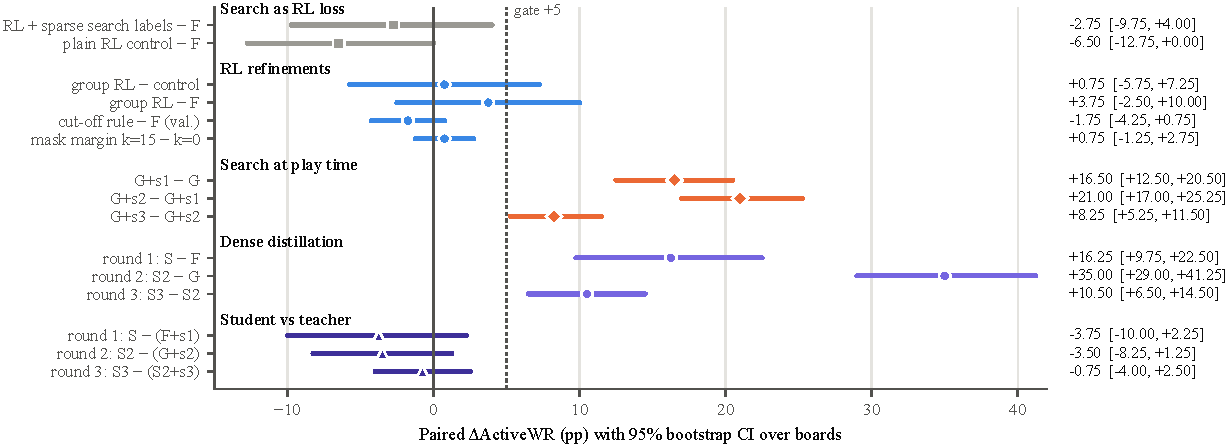
\includegraphics[width=\textwidth]{fig_forest.pdf}
\caption{Paired $\Delta$\awr{} with 95\% bootstrap CIs over boards, recomputed from per-game logs with the protocol's bootstrap seed; every value with a logged counterpart matches it exactly. Each group borrows the colour of the agent family it concerns. Dashed line: +5\pp{} gate. ``val.'' marks a validation-block comparison.}
\label{fig:forest}
\end{figure*}

\begin{figure*}[t]
\centering
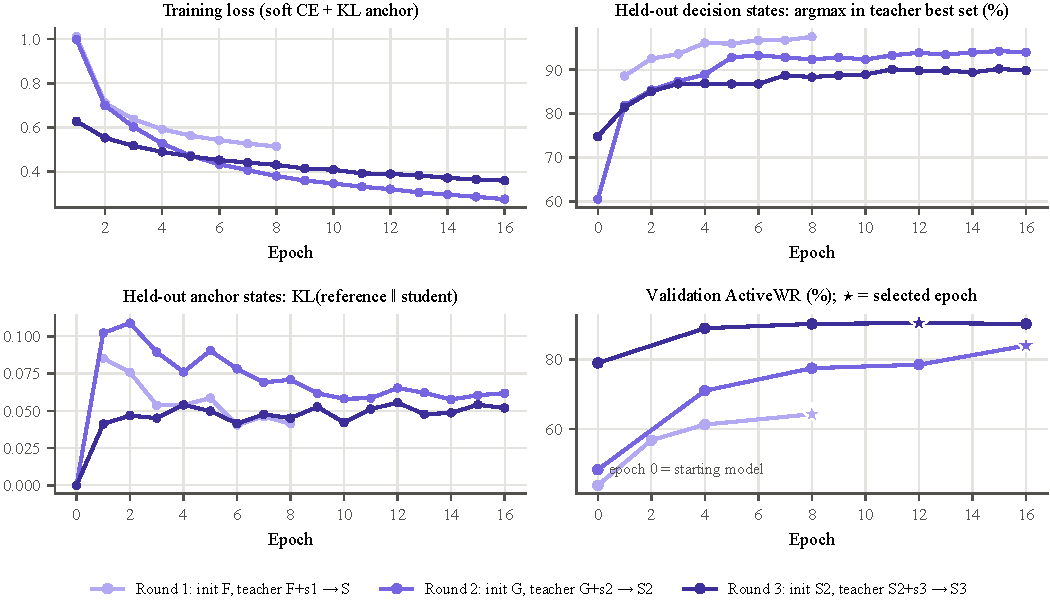
\includegraphics[width=\textwidth]{fig_distill_curves.pdf}
\caption{Distillation rounds, coloured by the student produced. Top left: training loss (soft-target cross-entropy plus the KL anchor). Top right: share of held-out decision states where the student's argmax is in the teacher's best set. Bottom left: KL from the reference (starting) policy on held-out anchor states. Bottom right: validation \awr{}; epoch 0 is the starting model and stars mark the epochs selected on validation before testing (8, 16 and 12). Held-out sets differ between rounds, so levels are comparable only within a round.}
\label{fig:distill}
\end{figure*}


\begin{figure}[t]
\centering
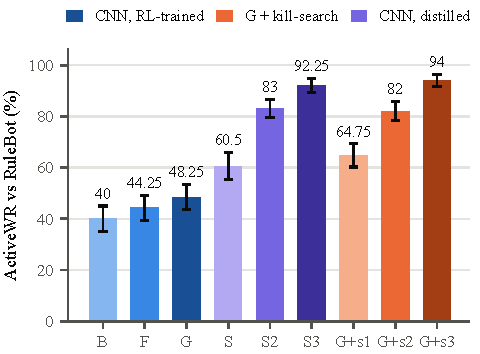
\includegraphics[width=\columnwidth]{fig_milestones.pdf}
\caption{\awr{} of every milestone (schedule E, 400 games each) with 95\% bootstrap CIs over boards. Each bar uses the model's own test block (Table~\ref{tab:main}), so differences between bars are descriptive. Colours identify agents throughout the paper.}
\label{fig:milestones}
\end{figure}

\begin{figure}[t]
\centering
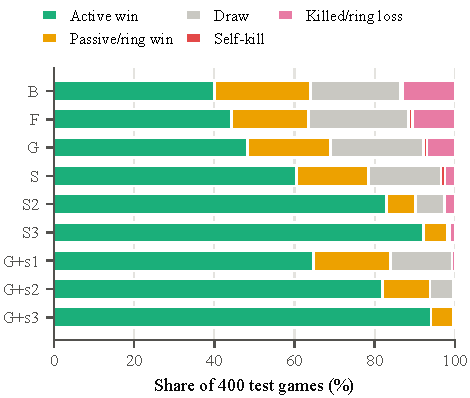
\includegraphics[width=\columnwidth]{fig_outcomes.pdf}
\caption{Outcome composition of the same 400-game tests. RL checkpoints win many games passively or by the ring; distilled students and search agents win by killing. Self-kills stay at or below 1\%.}
\label{fig:outcomes}
\end{figure}

\subsection{RQ1: win rate misjudges agents}
\label{sec:rq1}
Fig.~\ref{fig:wr} shows four interventions measured with both metrics on paired boards. A learner-side mask margin of $k=15$ steps for the shrinking ring raised WR by $+10.75$\pp{} \ci{6.25}{15.5} but \awr{} by only $+0.75$ \ci{-1.25}{2.75}; deaths in the ring fell from 116 to 76 of 400, so the gain was survival, not attack. A rule that makes the learner stand on the opponent's escape cell raised WR by $+3.75$ \ci{1.75}{6.0} while \awr{} fell by $1.75$ \ci{-4.25}{0.75}, with passive wins up from 9.5 to 15.25\%; owner-based credit shows that the rule turned 16 of F's active wins into passive ones. Turning sudden death on adds 16\pp{} of WR to G with no \awr{} change, and does nothing for S3, which wins before the ring starts. The earliest example is starker: a four-player checkpoint that passed our original WR gate (52.5\% over 40 games) had \emph{zero} kills with its own bombs. Evaluation only against RuleBot also overstates search agents: G+s3 reaches 94\% \awr{} against RuleBot (86--94\% in three- and four-player games) but only 8.5--20.5\% against frozen CNNs, with 50--70\% draws.

\begin{figure}[t]
\centering
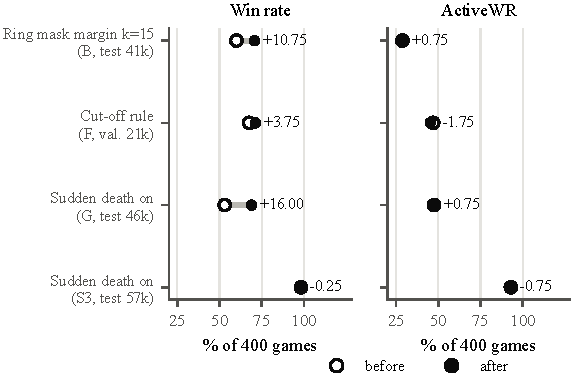
\includegraphics[width=\columnwidth]{fig_wr_vs_active.pdf}
\caption{Win rate versus \awr{} for the same paired games. Labels give after-minus-before in percentage points. WR gains come from passive or ring wins.}
\label{fig:wr}
\end{figure}

\subsection{RQ2: three uses of the same search}
Table~\ref{tab:three} compares three ways to use the depth-1 kill-search. As a sparse auxiliary loss inside RL (labels only where the search disagrees with the CNN, $\approx$0.9 labels per episode, each used once) it did not help: $-2.75$\pp{} \ci{-9.75}{4.0} over 3{,}000 episodes, no better than plain RL ($-6.5$ \ci{-12.75}{0.0}). At play time it adds $+16.5$\pp{} \ci{12.5}{20.5}. Densely distilled (about 6{,}200 decision states with counter-examples, 8 epochs), it moves the CNN by $+16.25$\pp{} \ci{9.75}{22.5}, nearly the play-time gain, with no search at play time. The distilled student learned the condition ``only BOMB kills here'': the probability of the best move on held-out decision states rose from 0.52 to 0.91, from 0.28 to 0.93 on states where the learner must stand in the escape cell, while $P(\text{BOMB})$ on ordinary states stayed at 0.088 $\rightarrow$ 0.095.

\begin{table}[t]
\centering
\caption{Three uses of the same depth-1 kill-search (paired \awr{} differences, own test blocks).}
\label{tab:three}
\scriptsize
\setlength{\tabcolsep}{3pt}
\resizebox{\columnwidth}{!}{%
\begin{tabular}{@{}llrl@{}}
\toprule
Use & Comparison & $\Delta$\awr{} [95\% CI] & Block \\
\midrule
Sparse auxiliary loss in RL & search arm $-$ F & $-2.75$ \ci{-9.75}{+4.0} & 42000 \\
Search at play time & G+s1 $-$ G & $+16.5$ \ci{+12.5}{+20.5} & 46000 \\
Dense distillation & S $-$ F & $+16.25$ \ci{+9.75}{+22.5} & 43000 \\
\bottomrule
\end{tabular}}
\end{table}

\begin{figure*}[t]
\centering
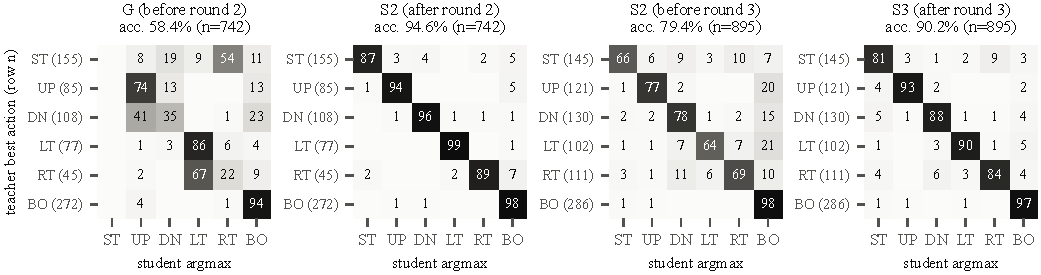
\includegraphics[width=\textwidth]{fig_confusion.pdf}
\caption{Action confusion on held-out decision states with a unique best action (rows: teacher's best action, with the number of states; columns: student argmax; row-normalised \%). Left pair: round 2 (teacher G+s2); right pair: round 3 (teacher S2+s3). ST/UP/DN/LT/RT/BO = STOP, UP, DOWN, LEFT, RIGHT, BOMB. Argmax on stored states, not sampled play; states with tied best actions (about 12\%) are excluded.}
\label{fig:confusion}
\end{figure*}

\begin{table*}[t]
\centering
\caption{Ablation study and controlled negative results (\awr{} in pp; paired over the stated block unless marked). Gate: $\Delta\ge+5$ and CI lower bound $>0$. ``val.'' = validation block 21000, descriptive only. Arms from B ran 200 episodes with learning rate $10^{-4}$ and were evaluated before sudden death existed; the sudden-death rows used an earlier ring schedule (start 400, interval 40). Arms from F ran 3{,}000 episodes with the defaults of Table~\ref{tab:hyper} and were evaluated under schedule E.}
\label{tab:ablation}
\scriptsize
\resizebox{\textwidth}{!}{%
\begin{tabular}{@{}llllrl@{}}
\toprule
Group & Change (one variable) & From & Block & $\Delta$\awr{} [95\% CI] & Outcome \\
\midrule
\multirow{8}{*}{RL refinements from B (200 ep)}
 & local attack teacher & B & 26000 & $+1.5$ \ci{-4.5}{7.25} & fail \\
 & two-bomb teacher & B & 26000 & $0.0$ (best = start) & fail \\
 & plain RL control (best ep.\ 400) & B & 32000 & $+2.25$ \ci{-3.25}{8.0} & fail \\
 & combat MOVE guidance & B & 33000 & $+5.25$ \ci{-1.5}{12.0} & fail (CI) \\
 & advantage normalisation & B & 34000 & $+0.25$ \ci{-5.5}{6.0} & fail \\
 & GAE ($\lambda=0.95$) & B & 35000 & $0.0$ (best = start) & fail \\
 & half wall reward & B & 36000 & $+0.5$ vs.\ B (35.0 vs.\ 34.5) & fail \\
 & PPO clip $\epsilon=0.2$, 4 epochs & B & 37000 & $-5.5$ (32.0 vs.\ 37.5) & fail \\
\midrule
\multirow{4}{*}{Sudden death}
 & train under SD, 12 channels & B & 40000 & $-2.25$ \ci{-8.0}{3.5} & fail \\
 & train under SD + ring channel & B & 40000 & $-2.25$ \ci{-7.5}{3.25} & fail \\
 & learner mask margin $k=15$ & B & 41000 & $+0.75$ \ci{-1.25}{2.75} (WR $+10.75$) & fail \\
 & rule teachers from step 360 & B & val. & $-4.25$ to $-2.25$ & fail \\
\midrule
\multirow{6}{*}{From F (3{,}000 ep)}
 & plain RL & F & 42000 & $-6.5$ \ci{-12.75}{0.0} & fail \\
 & sparse search labels in RL & F & 42000 & $-2.75$ \ci{-9.75}{4.0} & fail \\
 & argmax instead of sampling & F & val. & $-9.25$ \ci{-16.0}{-2.5} & worse \\
 & escape-cell cut-off rule & F & val. & $-1.75$ \ci{-4.25}{0.75} (WR $+3.75$) & fail \\
 & group advantage $K=8$, weight 1 & F & 44000 & $+0.25$ \ci{-5.75}{6.25} & fail \\
 & group advantage $K=16$, weight 4 (= G) & control & 45000 & $+0.75$ \ci{-5.75}{7.25} & fail \\
\midrule
\multirow{3}{*}{After distillation}
 & self-play RL vs.\ CNN pool, 2{,}000 ep & S2 & val. & 83.75 $\rightarrow$ 65.0 / 57.5 & skill lost \\
 & global KL anchor $\beta=1$, 500 ep & S2 & val. & 84 $\rightarrow$ 68 (control 76) & fail \\
 & search opponent model = own CNN & G+s3 & val. & $-33.0$ \ci{-41}{-25} vs.\ RuleBot & rejected \\
\midrule
\multirow{4}{*}{Accepted}
 & kill-search depth 1 at play time & G & 46000 & $+16.5$ \ci{12.5}{20.5} & pass \\
 & depth 2 vs.\ depth 1 & G+s1 & 47000 & $+21.0$ \ci{17.0}{25.25} & pass \\
 & depth 3 vs.\ depth 2 & G+s2 & 49000 & $+8.25$ \ci{5.25}{11.5} & pass \\
 & distillation rounds 1 / 2 / 3 & F / G / S2 & 43k/48k/57k & $+16.25$ / $+35.0$ / $+10.5$ & pass \\
\bottomrule
\end{tabular}}
\end{table*}

\subsection{RQ3: expert iteration with a network-free expert}
\textbf{Search depth.} Fig.~\ref{fig:depth} links depths on shared test blocks: depth 1 adds $+16.5$ over G, depth 2 adds $+21.0$ \ci{17.0}{25.25} over depth 1, and depth 3 adds $+8.25$ \ci{5.25}{11.5} over depth 2, nearly removing draws (5.75 $\rightarrow$ 0.25\%). The gains come from \emph{creating} a kill (step, then bomb) rather than finishing one: depth-1 search plateaus near 65\% whatever CNN it wraps (F, G or S).

\begin{figure}[t]
\centering
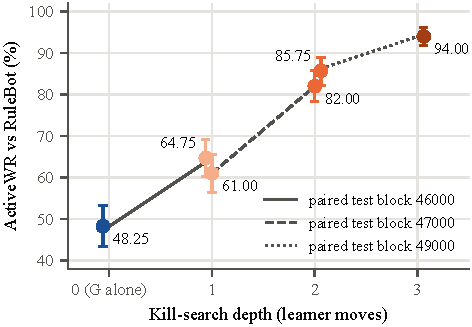
\includegraphics[width=\columnwidth]{fig_search_depth.pdf}
\caption{\awr{} versus kill-search depth around G. Marker colour identifies the agent; each line style joins the two agents tested on one paired block. Error bars: 95\% CIs over boards.}
\label{fig:depth}
\end{figure}

\textbf{Iterated distillation.} Each round closes most of the student--teacher gap (Fig.~\ref{fig:forest}, bottom group): S $-$ (F+s1) $=-3.75$ \ci{-10.0}{2.25}, S2 $-$ (G+s2) $=-3.5$ \ci{-8.25}{1.25}, S3 $-$ (S2+s3) $=-0.75$ \ci{-4.0}{2.5} (versus G+s3: $-1.75$), while the teachers get stronger. Round gains are $+16.25$ (S $-$ F), $+35.0$ \ci{29.0}{41.25} (S2 $-$ G) and $+10.5$ \ci{6.5}{14.5} (S3 $-$ S2). The S3 gain is active: passive wins change by $-1.5$ \ci{-4.5}{1.5}, draws by $-6.25$ \ci{-9.0}{-3.75}, games are shorter (131 versus 202 steps), and disabling sudden death gives the same $+10.75$ \ci{7.0}{14.5}. Round 3 is stable across training seeds: we repeated it twice with new collection boards and new train seeds, and on a shared fresh test block (400 games per model) the three S3 replicates beat S2 by $+10.5$ \ci{5.75}{15.25}, $+9.0$ \ci{4.25}{13.5} and $+9.25$ \ci{4.75}{13.75} (mean $+9.6$, s.d.\ 0.8); all three pass the gate. Fig.~\ref{fig:distill} shows the training signals: held-out agreement with the teacher's best set rises from 60.5 to 94.0\% in round 2 and from 74.8 to 89.8\% in round 3, while the KL to the reference policy on anchor states stays below 0.11 nats. Fig.~\ref{fig:confusion} gives the full action confusion on held-out decision states with a unique best action; in round 2 the main fix is movement: G often walks the opposite way to the search (LEFT in 67\% of states where RIGHT is best, UP in 41\% where DOWN is best) and almost never stops when STOP is best, while BOMB is already right in 94\% of cases. A stronger base does not make the search stronger: S2+s3 versus G+s3 on validation is $-5.0$ \ci{-11}{1}, consistent with a ceiling set by a search that ignores the network.

\textbf{Cost.} A search game takes 23--27\,s of CPU time against about 1\,s for CNN-only games; per decision, the depth-3 search costs \searchms{}\,ms on average against \cnnms{}\,ms for one S3 forward pass and sample (about \speedratio{}$\times$; 745 decisions in 6 validation games, one CPU thread, median 132 versus 1.8\,ms).

\subsection{RQ4: ablations and controlled negative results}
\label{sec:rq4}
Table~\ref{tab:ablation} collects every gated comparison; Fig.~\ref{fig:forest} plots the paired intervals recomputed from per-game logs. From B, 200-episode arms with teacher variants, curricula, advantage normalisation, GAE, reward changes and PPO clipping (evaluated before sudden death was added) all stayed within a few points of B; for GAE and the two-bomb teacher, validation kept the starting weights. Training under sudden death, with or without a ring channel, lowered \awr{} by 2.25\pp{}. From F, 3{,}000 more RL episodes did not help ($-6.5$), and neither did group-relative advantages on decisive states ($+0.75$ \ci{-5.75}{7.25} against the matched control), even though the latter raised the kill rate at those states by $+7.12$ \ci{4.86}{9.72}\pp{}; G is that checkpoint. Pushing BOMB at narrow states raised $P(\text{kill move})$ from 0.72 to 0.97 but not kills per game, and no KL weight separated ``bomb at the right moment'' from ``bomb anywhere''. Self-play RL against a pool of CNNs, starting from the distilled S2, erased the skill (\awr{} 83.75 $\rightarrow$ 65.0 and 57.5; agreement with the search 97.4 $\rightarrow$ 75.6 and 73.1\%), and a global KL anchor ($\beta=1$) kept only 2.5\pp{} of it. Fig.~\ref{fig:training} (Appendix) shows why RL from F is hard to read: rolling training \awr{} wanders between 35 and 55\% and validation peaks are not repeated on test.

\subsection{RQ5: draws between strong agents}
\label{sec:rq5}
Against frozen CNNs (S2, G, S3) S3 still draws 53--64\% of validation games, mostly at the 500-step limit (Fig.~\ref{fig:cnn}); against RuleBot it draws under 1\% with a median game length of 105 steps (Fig.~\ref{fig:length}, Appendix). S3 improves on S2 against CNNs by only $+3.33$ \ci{1.25}{5.50} \awr{} (macro over three opponents) and $-4.08$ \ci{-8.17}{-0.17} draws. To ask whether these draws hide missed kills, we replayed 195 draws of S3 and ran the depth-3 search at every fifth state with two opponent models (Fig.~\ref{fig:draws}). Under the RuleBot model the search sees a kill plan in 90.3\% of draws (2.98\% of states); with the opponent's own CNN as model it sees one in only 15.9\% \ci{9.9}{22.7} (0.19\% of states), while all 20 control active wins contain a plan. RuleBot-style traps are therefore mostly illusory against a CNN. Starting the ring earlier (step 400, 350 or 300) did not help either: \awr{} changed by $-1.42$ to $-0.17$\pp{}, and 80--87\% of the remaining draws became simultaneous deaths in the last ring. Conversely, a search that always models the opponent by a CNN gains against CNNs (+12.0 against F) but loses 33\pp{} against RuleBot. Both agents use the same safety mask, so neither steps into a forecast blast; a CNN dodges in varied ways and almost always keeps an exit, so a forced kill rarely exists.

\begin{figure}[t]
\centering
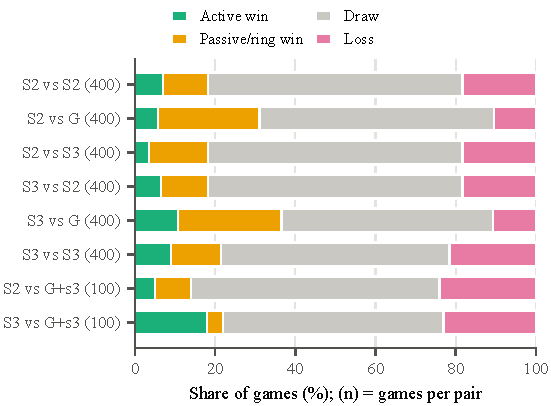
\includegraphics[width=\columnwidth]{fig_cnn_matchups.pdf}
\caption{Outcomes of CNN-versus-CNN and CNN-versus-search games on validation boards (learner listed first; games per pair in brackets). Outcome colours match Fig.~\ref{fig:outcomes}; passive/ring wins are mostly the opponent caught by the ring.}
\label{fig:cnn}
\end{figure}

\begin{figure}[t]
\centering
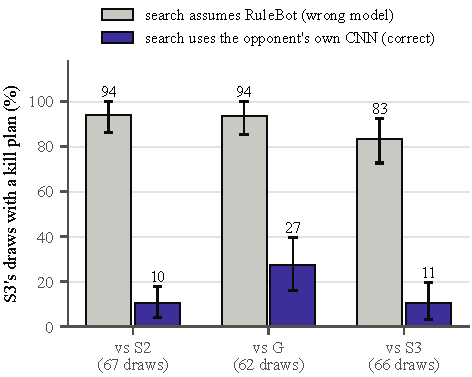
\includegraphics[width=\columnwidth]{fig_draw_probe.pdf}
\caption{Share of S3's draws against each CNN in which the depth-3 search finds a kill plan, under the wrong opponent model (RuleBot) and the correct one (the opponent's own CNN). Search runs at every fifth state. Error bars: 95\% bootstrap CIs over games.}
\label{fig:draws}
\end{figure}

\subsection{Transfer to an $11\times11$ board}
\label{sec:map11}
Interpolating S3's fully connected layer to $11\times11$ gives 46.25\% \awr{} on the larger board, whereas S3 + depth-3 search reaches 98\% on validation. One distillation round on 200 teacher games (746 decision and 1{,}310 anchor labels, 16 epochs) produced S3-11 with 87.25\% on a fresh test block, $+41.0$ \ci{34.5}{47.25}, with self-kills $+0.5$\pp{}. Against a pool of frozen CNNs (S3, S2, G; 2{,}400 games) S3-11 scored 8.58 versus 4.75\% macro \awr{}, $+3.83$ \ci{1.92}{5.83}, below the gate, with draws at 64.33 versus 63.08\%. Distillation transfers the RuleBot skill to a new board but does not resolve structural draws.

\subsection{Free-for-all against several RuleBots}
\label{sec:ffa}
On a fresh block (seed 50000, schedule E, 500 steps) one learner played against RuleBots in free-for-all. With three agents on $9\times9$ (60 boards $\times$ 3 seats, 180 games), G reached 27.2 \ci{21.1}{33.3} \awr{} (40.6\% WR) and G+s3 94.4 \ci{90.6}{97.8} (98.9\% WR). With four agents on $11\times11$ (40 boards $\times$ 4 seats, 160 games; the $9\times9$ network interpolated to the larger board), G reached 23.1 \ci{16.9}{29.4} (36.3\% WR, 53.8\% draws) and G+s3 86.3 \ci{80.0}{91.9} (88.8\% WR, 10.6\% draws). A RuleBot in the learner seat won 11.9\% (6.3\% \awr{}) and killed itself in 35.6\% of games.

The distilled students were then evaluated on a second fresh block (seed 59000, same protocol), with G re-run on the same boards so that the difference is paired. With three agents on $9\times9$, S3 reached 82.8 \ci{76.1}{88.9} \awr{} (87.8\% WR, 7.2\% draws, 0.6\% self-kills) against 36.1 for G, a paired difference of $+46.7$ \ci{+36.1}{+56.7}. With four agents on $11\times11$, interpolating S3 gave 25.0 \ci{18.1}{31.9}, not clearly above G (17.5; $+7.5$ \ci{-1.9}{+16.9}), whereas the $11\times11$ student S3-11 (Section~\ref{sec:map11}) reached 59.4 \ci{50.6}{68.1} \awr{} (63.8\% WR, 25.0\% draws), $+41.9$ \ci{+31.9}{+51.9} over G. Against fair shares of 33\% (three agents) and 25\% (four), 94\% and 93\% of the wins of S3 and S3-11 are active, against 64\% and 58\% for G: in free-for-all opponents also die by their own bombs, each other or the ring, so WR flatters weak agents most. Both students were distilled from 1v1 games only. G's \awr{} differs between the two blocks (27.2 versus 36.1 on $9\times9$), so the students are compared with G+s3 only descriptively: the gap to G+s3 grows from 1.75 points in 1v1 to about 12 points in three-agent free-for-all (94.4 on block 50000).

% =====================================================================================
\section{Discussion}

\textbf{Why dense distillation works where RL does not.} Decisive states are rare (in a 230-step game, about 2.2 steps where the search scores differ and 1.25 with a kill), and Monte-Carlo policy gradient spreads credit over all steps~\cite{williams1992reinforce}. A sparse label used once is too little signal; the same labels stored and replayed for several epochs, with counter-examples where BOMB is wrong, teach a conditional rule that RL's one-sided signal could not separate (Section~\ref{sec:rq4}). This matches the finding that more demonstrations matter more than better ones~\cite{kartal2019safer} and that policy distillation works best with sharp soft targets~\cite{rusu2016distill}.

\textbf{Why RL after distillation forgets.} Our anchors and KL penalties used fixed weights and pointed to the old student. Kickstarting~\cite{schmitt2018kickstart} needed a decaying weight to surpass the teacher, PPO found fixed-$\beta$ KL hard to tune~\cite{schulman2017ppo}, and imitation-then-PPO in Pommerman forgot catastrophically~\cite{meisheri2019}. Our measurement adds a reason: KL on decision states was about ten times larger than on ordinary states, so a global anchor is dominated by the states that do not matter. RL also mostly sharpened what F could already do: group-relative updates raised the kill rate by $+7.12$\pp{} at decisive states, and 86\% of those states were ones F converted in some but not all of 8 replays. This is in line with the observation that RL raises majority-vote accuracy but not pass@$k$~\cite{shao2024grpo}.

\textbf{The ceiling.} The search never uses the network, so expert iteration lacks ExIt's step where the apprentice improves the expert~\cite{anthony2017exit,silver2017agz}; S3 approaches but does not pass 94\%. Promising next steps, not yet tested, are: aggregating data across rounds and sampling fewer correlated states per game~\cite{anthony2017exit,ross2011dagger}; a search guided by S3's prior and value; pessimistic opponent scenarios~\cite{osogami2019} or a mixture of opponent models~\cite{lanctot2017psro} instead of one RuleBot model, which our probe shows overfits (a joint-policy-correlation effect); and RL anchored to the \emph{search teacher} on the student's own states with a decaying weight~\cite{schmitt2018kickstart}.

\textbf{How far the results generalise.} All agents were built and tested in one environment against one scripted opponent, and the search models that opponent. Three checks inside the environment show where the results hold. The student kept its skill in three-agent free-for-all, although it was distilled from one-versus-one games only (82.8\% \awr{}, Section~\ref{sec:ffa}). One more distillation round on $11\times11$ restored the skill on the larger board ($+41.0$\pp{}, Section~\ref{sec:map11}). Against frozen CNN opponents, however, both the search and its students lose most of their advantage (Section~\ref{sec:rq5}). The study therefore supports a claim about turning a search that models a known opponent into a fast network. It does not support a claim about strength against arbitrary opponents. The most direct external test is the official Pommerman free-for-all against SimpleAgent, which needs kicking and a 10-step fuse in both the simulator and the search, plus new distillation rounds.

\textbf{Draws.} High draw rates between strong agents are common in Pommerman~\cite{osogami2019,perezliebana2019,gao2019skynet}. Our probe separates draws that hide a kill under the right opponent model from draws where none exists, and suggests that changing the rules (a final ring that does not fill the board, longer games) would matter more than a stronger agent.

\begin{table*}[t]
\centering
\caption{Reported results of published Bomberman/Pommerman agents and of ours. Settings differ (Pommerman: $11\times11$, bombs explode after 10 steps, kicking, 800-step games, partial observation in team mode; ours: no kicking, 8-step bombs, 500-step games with sudden death, full observation), so rows position results and are not a head-to-head comparison. No published work reports \awr{}. FFA: free-for-all.}
\label{tab:sota}
\footnotesize
\setlength{\tabcolsep}{3pt}
\begin{tabular}{@{}L{0.14\textwidth}L{0.19\textwidth}L{0.15\textwidth}L{0.23\textwidth}L{0.23\textwidth}@{}}
\toprule
Work & Setting & Opponents & Method & Reported result \\
\midrule
Resnick 2018~\cite{resnick2018pommerman} & Pommerman FFA, 4 agents & 3 SimpleAgents & reference level & an agent as strong as SimpleAgent wins $\approx$20\% \\
Gao 2019~\cite{gao2019hard} & Pommerman FFA / team & 3 SimpleAgents / SimpleAgent team & PPO + action pruning & WR 40--43\% (FFA), 65--76\% (team); $3\times100$ games \\
Perez-Liebana 2019~\cite{perezliebana2019} & Pommerman FFA, full observation & 3 rule-based agents & MCTS / RHEA & WR 46.5\% / 33.0\% \\
Weil 2023~\cite{weil2023} & official Pommerman FFA & 3 SimpleAgents & MCTS + learned model (ExIt-style) & WR 61--78\%, ties 12--34\% (5 models, 100 games each) \\
Meisheri 2019~\cite{meisheri2019} & Pommerman team $2\times2$, partial & SimpleAgent team & imitation $\rightarrow$ PPO & WR 77.8\% \\
Osogami 2019~\cite{osogami2019} & Pommerman team $2\times2$ & SimpleAgent team & depth-1 tree search, pessimistic scenarios & WR 92.6--99.7\% (pessimism level 0--3) \\
Huynh 2024~\cite{huynh2024} & Pommerman team $2\times2$, partial & SimpleAgent team; search agent dypm & PPO + LSTM, curriculum, population self-play, 200M steps & WR 98.85\% vs SimpleAgent; 30.0\% vs dypm \\
\midrule
Ours, G & FFA $11\times11$, 4 agents & 3 RuleBots & masked PG + group advantage & WR 36.3\%, \awr{} 23.1\% (160 games) \\
Ours, G+s3 & FFA $11\times11$, 4 agents & 3 RuleBots & G + network-free kill-search & WR 88.8\%, \awr{} 86.3\% (160 games) \\
Ours, S3-11 & FFA $11\times11$, 4 agents & 3 RuleBots & distilled CNN, no search at play time & WR 63.8\%, \awr{} 59.4\% (160 games) \\
Ours, S3 & FFA $9\times9$, 3 agents & 2 RuleBots & distilled CNN, no search at play time & WR 87.8\%, \awr{} 82.8\% (180 games) \\
Ours, G+s3 & 1v1 $9\times9$ & RuleBot & G + network-free kill-search & WR 99.5\%, \awr{} 94.0\% (400 games) \\
Ours, S3 & 1v1 $9\times9$ & RuleBot & distilled CNN, no search at play time & WR 98.0\%, \awr{} 92.25\% (400 games) \\
\bottomrule
\end{tabular}
\end{table*}

\textbf{Comparison with published agents.} No agent was run in both environments, so Table~\ref{tab:sota} positions results rather than ranking them. Pommerman is the broader benchmark (larger board, four agents, kicking, partial observation in team mode), but three differences make our numbers conservative. \emph{First, the criterion is stricter.} Every published result counts all wins, including games in which opponents killed themselves; our headline number counts only kills credited to the agent's own bombs. Under the published criterion S3 would report 98.0\% instead of 92.25\%, and G+s3 88.8\% instead of 86.3\% in four-agent free-for-all. \emph{Second, waiting is not rewarded.} Bombs explode after 8 steps instead of 10, and a closing ring shrinks the arena near the end, whereas in Pommerman most ties come from games that reach the 800-step limit~\cite{weil2023}. \emph{Third, the budget is small.} S3 was trained and distilled on consumer machines and needs one forward pass per move, 0.75 points below its search teacher; the strongest learning agent in Pommerman needed 200 million steps of population-based self-play and still wins only 30\% against a depth-1 tree search~\cite{huynh2024,osogami2019}. Within these caveats the ordering matches the Pommerman literature: search leads learning (our RL checkpoints reach 40.0--51.0\% \awr{}, G+s3 94.0\%), and in the setting closest to Pommerman free-for-all (four agents on $11\times11$, Section~\ref{sec:ffa}) G+s3 wins 88.8\% against three RuleBots and the network-only S3-11 63.8\%, compared with 40--43\% for PPO~\cite{gao2019hard} and 61--78\% for MCTS with learned models~\cite{weil2023} against three SimpleAgents. Both reference bots are weak heuristics below the fair share (11.9\% for RuleBot, about 20\% at SimpleAgent level~\cite{resnick2018pommerman}) but were never played against each other, and our students were distilled and evaluated only against RuleBot. \awr{} itself has no published counterpart; the closest is Skynet's observation that wins often came from opponents killing themselves~\cite{gao2019skynet}.

% =====================================================================================
\section{Limitations}
(1) Only distillation round 3 was replicated over training seeds (three seeds, all passing the gate); the earlier rounds and the RL arms used one seed, so their intervals measure variation over evaluation boards, not over training runs~\cite{henderson2018matters,agarwal2021precipice}. (2) The reference opponent is RuleBot, and the search assumes RuleBot; S3 is strongest against it and only slightly better than S2 against CNNs. (3) Milestones in Table~\ref{tab:main} come from different test blocks; one block varies by about $\pm5$\pp{}. B's row uses a cross-check block because its original test predates sudden death, and the 200-episode ablations from B were also evaluated without it. (4) Policies are sampled, so numbers reproduce bit-for-bit only with the same torch version; validation results from different torch versions are not compared. (5) Most results are 1v1 on $9\times9$; free-for-all and $11\times11$ results are single runs. (6) Some arms (F, S, S2, the self-play and KL-anchor runs) were trained on a second machine. (7) Of the 35 core references, one~\cite{goulart2019} was consulted only as an abstract, so its result is not listed in Table~\ref{tab:sota}. (8) Our agents were not run in the official Pommerman environment (kicking, 800-step games, team mode with partial observation) or against SimpleAgent, so Table~\ref{tab:sota} positions rather than compares; running S3 and G+s3 there is the most direct next test.

% =====================================================================================
\section{Conclusion}
In Bomberman, win rate rewards survival and opponent mistakes; \awr{} measures what we want, an agent that wins by killing. Measured this way, model-free RL with a safety mask stalls below about 50\%, while a short, network-free kill-search reaches 94\%. Storing the search's labels on decision states and distilling them, three times over, gives a single CNN at 92.25\% that needs one forward pass per move. Against equally careful neural opponents most games remain draws, and our probe indicates that this comes mainly from the game's rules.

% =====================================================================================
\section*{Statements}
\noindent\textbf{Data and code availability.} Environment, training, search and evaluation code, the pre-specified run registrations, per-game evaluation logs and the scripts that produce every figure (\texttt{paper/scripts}) are in the authors' repository. An anonymised copy is provided for review at \url{https://anonymous.4open.science/r/ANONYMOUS-ID}; the public repository will be linked in the camera-ready version.
% TODO before submission: create the anonymised mirror of the GitHub repository at anonymous.4open.science and replace ANONYMOUS-ID.

\noindent\textbf{Ethics.} The study uses simulated games only and no human data.

\noindent\textbf{Funding and competing interests.} This work received no external funding; it was carried out as a student project. The authors declare no competing interests.

\noindent\textbf{Author contributions (CRediT).} Author 1 (first author): conceptualization, methodology, software, investigation, formal analysis, visualization, writing -- original draft. Authors 2 and 3: [roles to be completed by the authors, e.g.\ software, investigation, validation, writing -- review and editing]. All authors approved the final manuscript. Names are withheld for double-anonymous review.

\noindent\textbf{Use of AI tools.} An AI assistant was used to help draft and edit the text and to write plotting code; the authors designed the experiments, ran them, checked every number against the logs and take responsibility for the content.

\bibliographystyle{IEEEtran}
\bibliography{references}

% =====================================================================================
\appendix
Figs.~\ref{fig:obs}--\ref{fig:training} show the observation planes, game lengths and RL training curves.

\begin{figure*}[t]
\centering
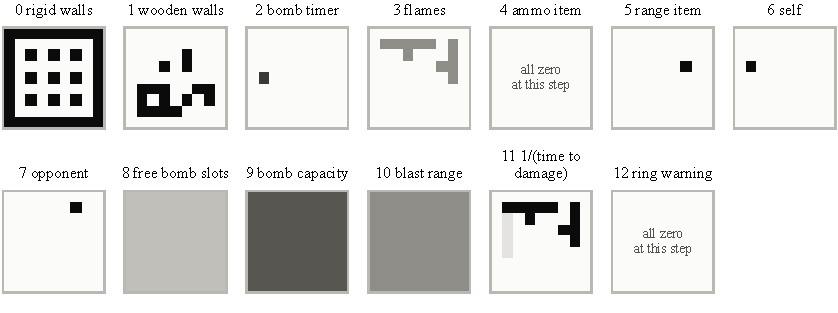
\includegraphics[width=\textwidth]{fig_observation.pdf}
\caption{The 13 observation planes for one agent (validation board 21007, step 26, RuleBot vs RuleBot; darker = larger). The agent has collected one ammo item (capacity 2 of 3) and has one bomb on the board, so one slot is free; a range item lies on the board. Planes marked ``all zero'' are empty at this step: no ammo item is visible, and the ring warning starts 40 steps before the first closure.}
\label{fig:obs}
\end{figure*}

\begin{figure*}[t]
\centering
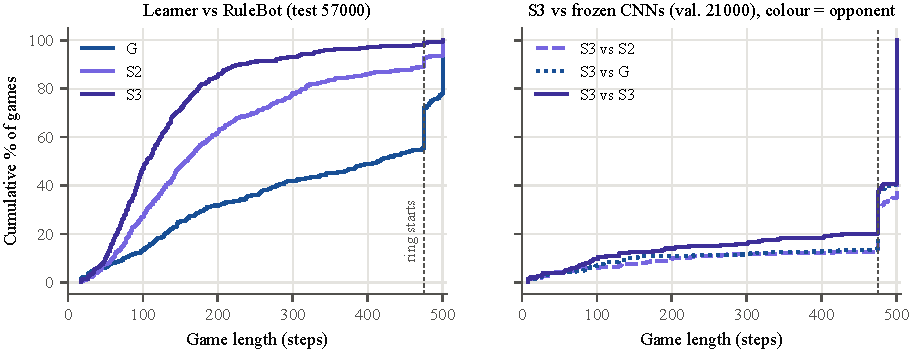
\includegraphics[width=\textwidth]{fig_episode_length.pdf}
\caption{Cumulative distribution of game length. Against RuleBot, stronger agents finish earlier (median 414, 158 and 105 steps for G, S2, S3; 22.25, 6.5 and 0.75\% reach the limit). Against frozen CNNs (right; colour = opponent), 59.5--65\% of S3's games reach 500 steps. The left panel uses test block 57000, the right one validation block 21000.}
\label{fig:length}
\end{figure*}

\begin{figure*}[t]
\centering
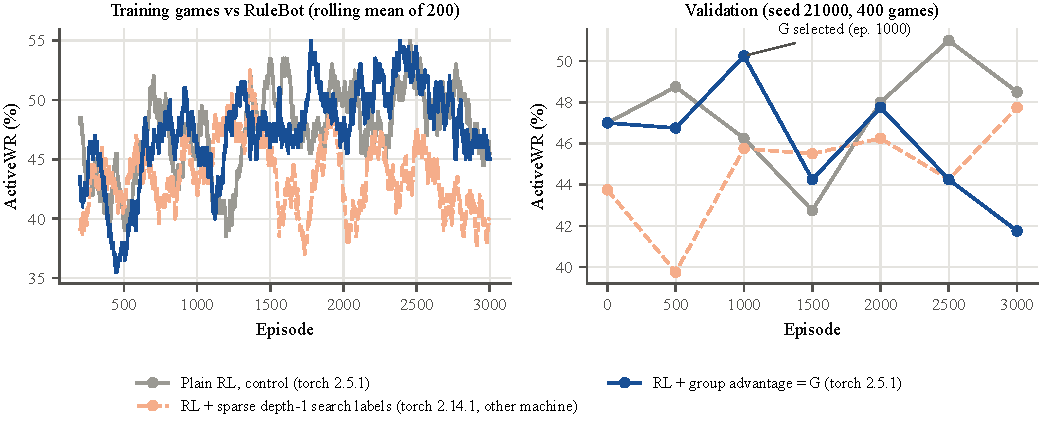
\includegraphics[width=\textwidth]{fig_training_curves.pdf}
\caption{RL from F (3{,}000 episodes per arm, one train seed). Left: rolling \awr{} of training games against RuleBot. Right: validation \awr{} every 500 episodes. The group-advantage arm peaked at episode 1000 (50.25) and became G; on the test block it was $+0.75$ over the control. The dashed arm ran on a second machine with torch 2.14.1; because actions are sampled, its validation numbers are not comparable with the other two (the same F scores 43.75 there versus 47.0 at episode 0). Its test result (Table~\ref{tab:three}) was re-run on the same machine as the others.}
\label{fig:training}
\end{figure*}

\end{document}
